\begin{song}{title=\predtitle\centering Ráda se miluje \\\large Karel Plíhal  \vspace*{-0.3cm}}  %% sem se napíše jméno songu a autor
\begin{centerjustified}
\nejnejvetsi

\refren
^{Hmi}Ráda se miluje, ^{A{\color{white}\_}}ráda ^{D\,}jí,

^{G{\color{white}\_}}ráda si ^{F#mi\,}jenom tak ^*{Hmi}zpívá ,

^{Hmi\z}vrabci se na plotě ^{A\,{\color{white}\_}D\,}hádají,

^*{G}ko lik ^{\,\,F#mi}že~času~jí ^{Hmi\z}zbývá.

\sloka
^{G}Než vítr dostrká k ^{D\z}útesu ^{G\z}tu~její ^{\z D\,\,F#mi}legrační~bárku~~~~

a ^{Hmi\z}Pámbu si ve svým ^{A\z D}notesu ^{G\z F#mi\:\:\:\:\:\:}udělá~jen~další ^{Hmi\z}čárku.

\refren

\sloka
^{G\z}Psáno je v nebeské ^{D\z}režii, ^{G\z}a~to hned na ^{\z D\,\,F#mi}první~stránce,~

že ^{Hmi\z}naše duše nás ^{A\z D}přežijí ^{G\z}v~jinačí ^{F#mi\z}tělesný ^{Hmi\z}schránce.

\refren

\sloka
^{G\z}Úplně na konci ^{D\z}paseky, ^{G\z}tam, kde se ^{\z D\,\,F#mi}ozvěna~tříští,~~~~

^{Hmi\:}sedí~šnek ve snacku ^{A\z D}pro~šneky -- ^{G\z}snad její ^{F#mi\z}podoba ^{Hmi\z}příští.


\refren

\end{centerjustified}
\setcounter{Slokočet}{0}
\end{song}

\begin{figure}[h]
\predtitle\centering
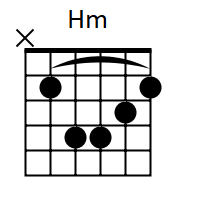
\includegraphics[width=3cm]{../Akordy/hm.png}
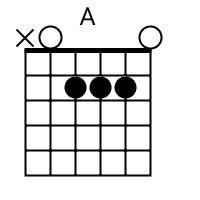
\includegraphics[width=3cm]{../Akordy/a.png}
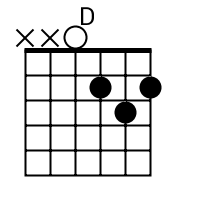
\includegraphics[width=3cm]{../Akordy/d.png}
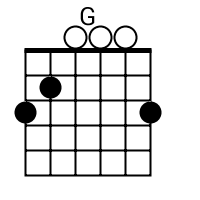
\includegraphics[width=3cm]{../Akordy/g.png}
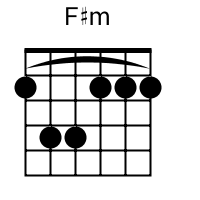
\includegraphics[width=3cm]{../Akordy/fxm.png}
\end{figure}
